\section{Translating Experimental Results to Pebble Bed Interactions}\label{sec:theoryStrainEnergy}

It is impractical, if not impossible, to accurately measure the contact forces between all the pebbles in a densely-packed, three-dimensional ensemble. In investigating the probability of pebbles becoming damaged (i.e. crushed or cracked) in a packed bed, we therefore rely on the combined information gained from indirect measurements of the entire pebble bed, crush experiments of individual pebbles, and the predictive capabilities of DEM simulations. In this study we look at the results of individual pebble crush experiments and create a metric to link the data to the contact forces measured in DEM to help predict when pebbles in the ensemble will become damaged.

\subsection{Experimental Measurements of Strain Energy}
\begin{figure}[!t]
\centering
    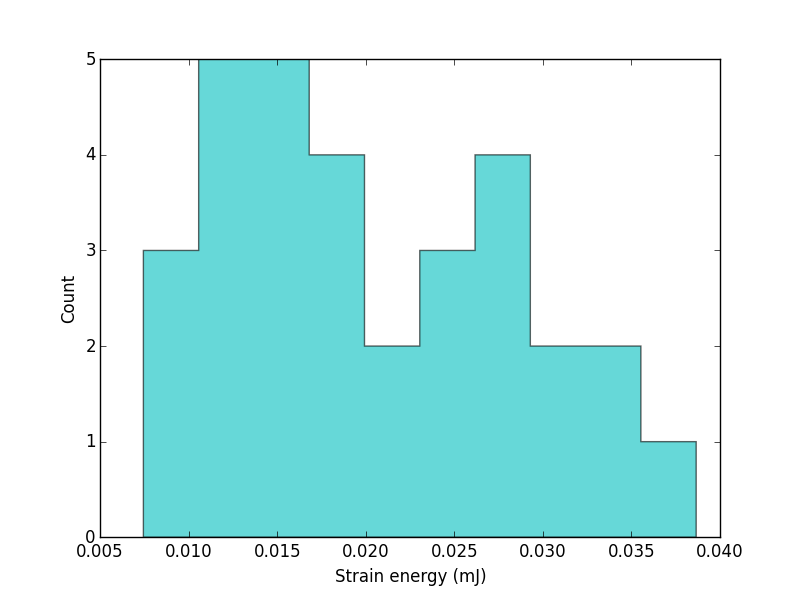
\includegraphics[width=\doubleimagewidth]{chapters/figures/fzk-w-histogram.png}
    \caption{Histogram of the absorbed strain energy at the moment of crushing for \lis pebbles as measured in single pebble crush experiments.}
    \label{fig:fzk-w-hist}
\end{figure}

\begin{figure}
        \centering
        \begin{subfigure}[b]{\doubleimagewidth}
                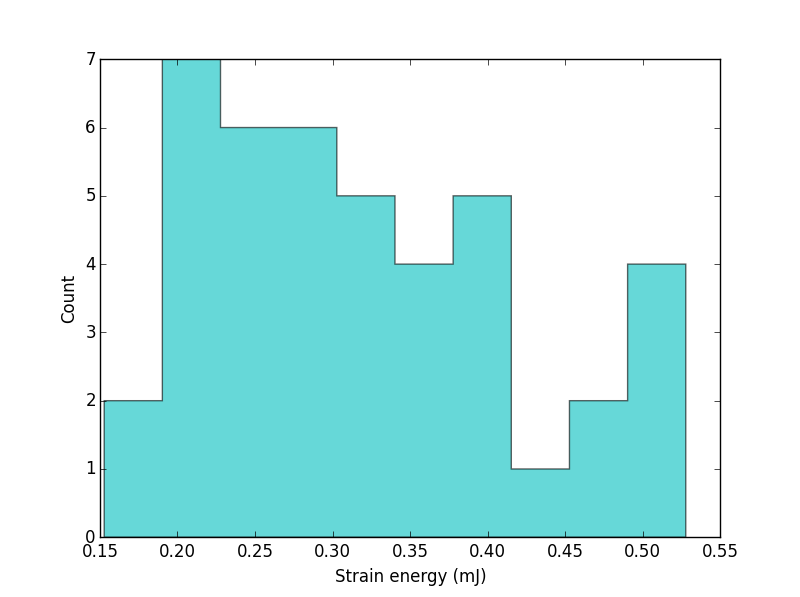
\includegraphics[width=\textwidth]{chapters/figures/nfri-1mm-w-histogram.png}
                \caption{$\bar{d}_p = 1$ mm}
                \label{fig:nfri-1-w-hist}
        \end{subfigure}
        ~
        \begin{subfigure}[b]{\doubleimagewidth}
                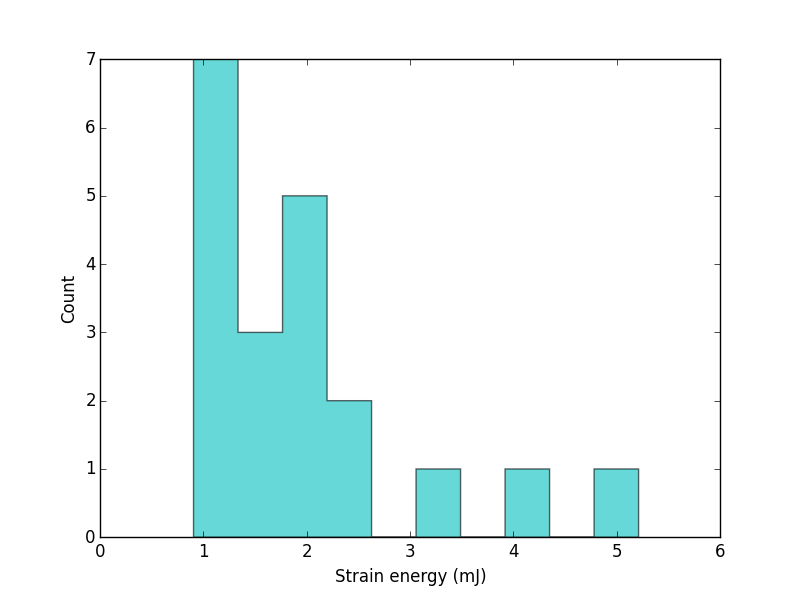
\includegraphics[width=\textwidth]{chapters/figures/nfri-1.5mm-w-histogram.png}
                \caption{$\bar{d}_p = 1.5$ mm}
                \label{fig:nfri-1.5-w-hist}
        \end{subfigure}
        \caption{Histogram of the absorbed strain energy at the moment of crushing for \lit pebbles as measured in single pebble crush experiments.}\label{fig:nfri-w-hist}
\end{figure}

The normal force between two elastic objects is a function of the material properties of the interacting objects (see Eq.~\ref{eq:hertz-normal-force}). We cannot, therefore, directly compare the forces between pebble-test stand with pebble-pebble in an ensemble. An approached used by some solid breeder researchers is to relate the absorbed strain energy of the pebble\cite{Zhao2013,Annabattula2012a}. We integrate the Hertzian force along the overlap to find the strain energy, $W_\epsilon$, of that contact. 

\begin{equation}\label{eq:strain-energy-integral}
	W_\epsilon = \int_0^{\delta_c}\!F_n(\delta')\,\mathrm{d}\delta'
\end{equation}
where the upper limit of the integration is the critical overlap $\delta_c$. Inserting Eq.~\ref{eq:hertz-normal-force} into Eq.~\ref{eq:strain-energy-integral},
\begin{align}
	W_\epsilon& = \int_0^{\delta_c}\!  \frac{4}{3}E^*\sqrt{R^*}\,\delta'^{3/2} \,\mathrm{d}\delta' \\
	%W_\epsilon & = \frac{4}{3}E^*\sqrt{R^*} \left[\frac{2}{5}\,{\delta_c}^{5/2}\right] \\
	W_\epsilon & = \frac{8}{15}E^*\sqrt{R^*}\, {\delta_c}^{5/2}
\end{align}

We will call the strain energy of the pebble compressed between platens as the lab strain energy, $W_{\epsilon,L}$. In pebble crushing experiments, we record the strain energy absorbed up to the point of crushing, the data for \lis and \lit pebbles are given in Figs.~\ref{fig:fzk-w-hist} and~\ref{fig:nfri-w-hist}, respectively. Then the strain energy of two particles in contact will be $W_{\epsilon,B}$. The assumption we make is that, if each contact interaction is integrated to the proper critical overlap, the strain energies will be equal at that contact.

\begin{equation}
	W_{\epsilon,L} = W_{\epsilon,B} = \frac{8}{15}E_B^*\sqrt{R_B^*}\, {\delta_{c,B}}^{5/2}
\end{equation}

We solve for the interacting pebble bed overlap as a function of the lab strain energy as

\begin{equation}
	\delta_{c,B} = \left[\frac{15W_{\epsilon,L}}{8E_B^*\sqrt{R_B^*}}\right]^{2/5}
\end{equation}

This overlap can be reinserted to the Hertz force of Eq.~\ref{eq:hertz-normal-force} to find the critical force (crush force) of the interacting particles as a function of the critical strain energy of the lab. Doing this, we find,
\begin{equation}\label{eq:peb_hertz}
	F_{c,B} = C{E_B^*}^{2/5}{R_B^*}^{1/5}W_{\epsilon,L}^{3/5}
\end{equation}
where $C = \frac{4}{3}\left(\frac{15}{8}\right)^{3/5}$.

Equation~\ref{eq:peb_hertz} is a generic translation between lab materials and packed bed materials. We will use the equation as the basis for our pebble crushing prediction in DEM simulations.





% FROM SOFT PAPER
\subsection{Calculating Critical Strain Energy}
With the rise of micro-mechanical tools and computing power, attempting to predict when ceramic pebbles will crush in an ensemble, based on inter-particle contact forces, has received considerable attention. In this section we will review literature studying granular crushing.

Probability and statistics were applied to the study of packed beds of brittle grains by Marketos and Bolton\cite{Marketos2007}. The fundamental assumption in their predictive method was the independence of crushing events. They used their model to predict the initiation of crushing as well as the evolution of the packing after crushing. They created somewhat arbitrary probability distributions of the strength of their granular particles,
\begin{equation}
	h(\Phi) = \frac{0.0395}{\sqrt{\Phi}}
\end{equation}
where $\Phi$ is a characteristic strength parameter falling between 160 and 640~N. The form of their distribution was based on single crushing tests on quartz particles from Nakata\etal.

A common alternative distribution is to use a form first proposed by Weibull for a material under uniform stress\cite{Kwok2013,Zhao2011,nakata1999probabilistic,Zhao2013,Pitchumani2004}. The form, as written by Zhao\etal~is,
\begin{equation}
	P_s = 1 - \exp\left[-\left(\frac{W_c}{W_\text{mat}}\right)^m\right]
\end{equation}
where $W_c$ is the energy absorbed by the pebble and $W_\text{mat}$ and $m$ characterize the material. An important note is how to calculate the critical strain energy for the pebble. Refs.~\cite{Marketos2007} and \cite{Zhao2011} note the necessity to consider the coordination number dependence on total strain energy. In other words, the total strain energy is the cumulative total of strain energy at every contact. Zhao\etal~give strain as
\begin{equation}
	W_c = \sum_{i=1}^{Z_i}\left(\frac{9}{80 R_{ij}^*}\right)^{1/3} \left(\frac{1}{E_{ij}^*}\right)^{2/3} F_{n,ij}^{5/3}
\end{equation}
where $Z$ is the coordination number of pebble $i$. 

However, Russell\etal, analyzed ideal granular assemblies for which they could find analytical solutions to stress distributions inside of pebbles.\cite{Russell2009} In their work, failure of a granular particle initiates at the location of maximum of the stress invariant ratios. In the contact of elastic spheres, the stress fields near the contact areas are highly localized. Because of the highly localized effects, Russell\etal~find that in granular assemblies the contributions to failure initiation are not additive. They discovered that the initiation of failure is always located adjacent to the largest force irrespective of the material properties or geometric size of the pebbles in an ensemble. Russell\etal\cite{Russell2009} conclude: the largest contact force acting upon a particle is the primary agent driving the damage of the individual. Based upon the failure criterion developed for brittle materials, crushing of an individual does not directly depend upon the presence or magnitude of any lesser contact forces acting on the particle or the material properties of the particle. Although their results were obtained for idealized assemblies, the results are generally true for any situation where multiple contact forces are present.

\begin{figure}[!t]
\centering
    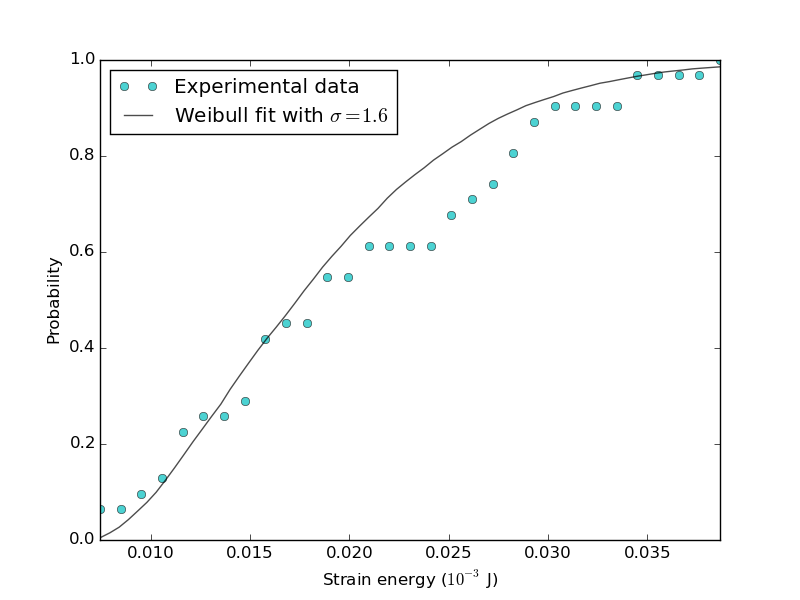
\includegraphics[width=\doubleimagewidth]{chapters/figures/fzk-w-cdf-fit.png}
    \caption{Fitting the strain energy with a Weibull distribution with shape parameter specific for the \lis pebbles.}
    \label{fig:fzk-w-cdf}
\end{figure}

\begin{figure}
        \centering
        \begin{subfigure}[b]{\doubleimagewidth}
                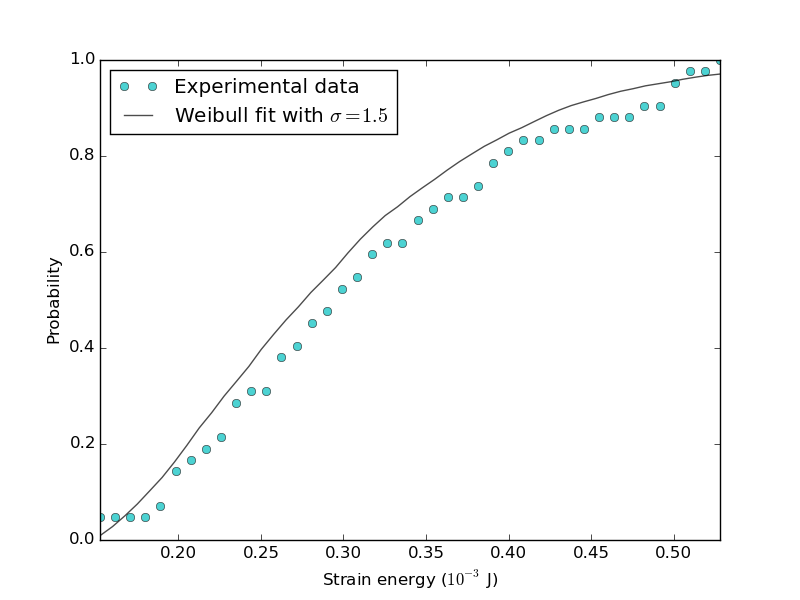
\includegraphics[width=\textwidth]{chapters/figures/nfri-1mm-w-cdf-fit.png}
                \caption{$\bar{d}_p = 1$ mm}
                \label{fig:nfri-1-w-cdf}
        \end{subfigure}
        ~
        \begin{subfigure}[b]{\doubleimagewidth}
                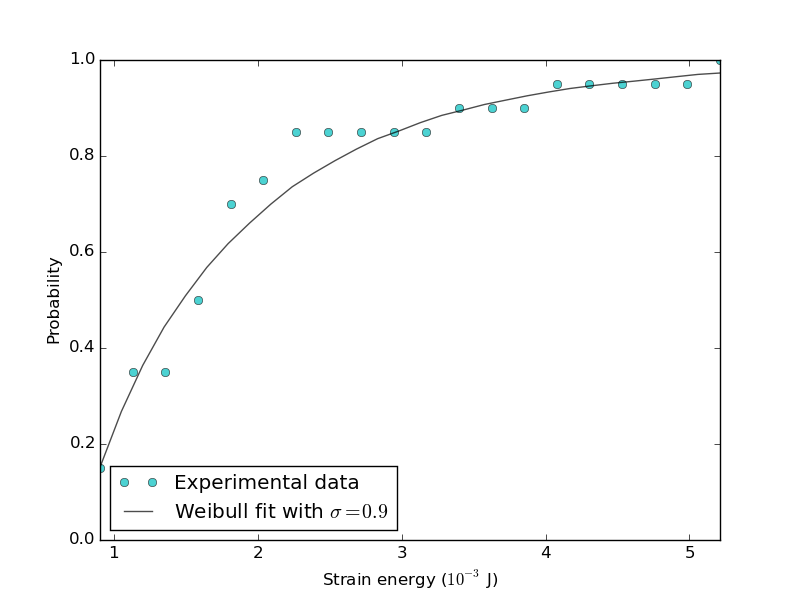
\includegraphics[width=\textwidth]{chapters/figures/nfri-1.5mm-w-cdf-fit.png}
                \caption{$\bar{d}_p = 1.5$ mm}
                \label{fig:nfri-1.5-w-cdf}
        \end{subfigure}
        \caption{Fitting the strain energy with a Weibull distribution with shape parameter specific for the two batches of \lit pebbles.}\label{fig:nfri-w-cdf}
\end{figure}

Based on the compelling arguments of Russell\etal, we will define our critical force as the maximum contact force on the pebble in our assembly,
\begin{equation}
	F_{c} = \max F_{n,ij}
\end{equation}

Then we can say a pebble is crushed when the force on the pebble in the bed is greater than the critical bed force defined from Eq.~\ref{eq:peb_hertz},

\begin{equation}\label{eq:crush-predict}
  F_{c} > F_{c,B} = \frac{4}{3}\left(\frac{15}{8}\right)^{3/5}{E_B^*}^{2/5}{R_B^*}^{1/5}W_{\epsilon,L}^{3/5}
\end{equation}

In the implementation into DEM, the probabilistic features appear naturally in this formulation from the measured probability distribution of $W_{\epsilon,L}$. In the experiments on crushing individual pebbles, the critical strain energy is measured strain energy at the point of crushing. This value follows a probability distribution and therefore imparts a distribution shape to the $F_{c,B}$ prediction. Cumulative distribution functions are generated for the strain energy data (see Figs.~\ref{fig:nfri-w-hist} and~\ref{fig:nfri-w-hist}). From that data, we fit Weibull distribution curves, of the form
\begin{equation}
	\Xi = \lambda\left[-\ln(W_\epsilon)\right]^{1/\sigma}
\end{equation}
where the shape parameter, $\sigma$, is fit to the specific curve of each set of experimental data and the second parameter, $\lambda$ is
\[
\lambda = \bar{W}_\epsilon - \min W_\epsilon
\]

In Figs.~\ref{fig:fzk-w-cdf} and~\ref{fig:nfri-w-cdf} we show the experimental data and the Weibull fits specific to the ceramic material and batch. The Weibull distribution functions will be used again when we generate strength parameters to assign to pebbles in the discrete element simulations of pebble crushing, addressed in \cref{sec:failure-study}.